\section{函数的性质}
\label{sec:prelim-optimal-values-errors}
\label{sec:ru-function-properties}

从候选函数中挑选时，常把每个候选的优劣写成一个实数，再寻找使它最小的候选。这要求我们能够描述一个函数的取值范围、增减方向和对称性，
并分清“最小的值是多少”和“在哪里取到”。本节把实数集合的确界用到函数的像集上，再用输入之间的关系定义单调、奇偶和周期。

设$X$非空，$f:X\to\mathbb R$。函数的有界性就是像集$f(X)$的有界性：若$f(X)$有上界，称$f$上有界，下界与有界同理。
像集的确界简记为
\[
 \sup_{x\in X}f(x)=\sup f(X),\qquad \inf_{x\in X}f(x)=\inf f(X).
\]
若$f(X)$无上界，约定$\sup_Xf=+\infty$；若无下界，约定$\inf_Xf=-\infty$。这两个符号只表示没有有限的界，不是函数实际取到的数。
若存在$x^\star\in X$使$f(x^\star)=\inf_Xf$，就称$f(x^\star)$为$f$的最小值；最大值类似。
例如$f(x)=x$在$(0,1)$上有下确界$0$，却没有最小值：任一允许的输入$x$都有更小的允许输入$x/2$。

若对$X$中任意$x<y$都有$f(x)\leq f(y)$，称$f$单调不减；若总有$f(x)<f(y)$，称$f$严格递增。
单调不增与严格递减类似地定义，它们统称\term{单调函数}（monotone function）。单调性比较的是两个输入及其输出的大小关系，与函数能否用公式写出无关。

奇偶性与周期性描述输入变换下函数值的不变性。若定义域关于原点对称（$x\in X$蕴含$-x\in X$），并且$f(-x)=f(x)$，称$f$为偶函数，图像关于纵轴对称；
若$f(-x)=-f(x)$，称$f$为奇函数，图像关于原点对称。定义域不对称时谈不上奇偶：$x^2$在$[0,1]$上不是偶函数，因为$-1/2$不在定义域中。
若存在$T>0$，使$x\in X$蕴含$x+T\in X$且$f(x+T)=f(x)$，称$f$以$T$为周期；平移输入$x\mapsto x-c$则把图像整体右移$c$。
这些性质都依赖定义域，讨论时须把定义域与表达式一起写明。

严格单调还带来可逆性。若$f$在$X$上严格递增，则$x\neq y$时$f(x)\neq f(y)$，$f$是$X$到像集$f(X)$的双射，因而有反函数$f^{-1}:f(X)\to X$。
反函数仍严格递增：若$u<v$属于$f(X)$而$f^{-1}(u)\geq f^{-1}(v)$，两边作用$f$便得$u\geq v$，矛盾。
这里只得到了反函数的存在与单调性；反函数是否连续，要等下一章有了连续性的概念才能讨论。

\paragraph{最小值与最小点}
寻找最小值时，答案包含两部分：最小的函数值是多少，以及哪些输入取到它。若$x^\star\in X$满足
\[
 f(x^\star)\leq f(x)\qquad\text{对所有}\ x\in X,
\]
则称$x^\star$为\term{全局最小点}（global minimizer），$f(x^\star)$为最小值，记作$\min_{x\in X}f(x)$。全部最小点组成的集合记作
\[
 \argmin_{x\in X}f(x)=\{x\in X:\ f(x)\leq f(z)\ \text{对所有}\ z\in X\}.
\]
$\min$给出一个数，$\argmin$给出输入的集合；若不存在最小点，后一个集合为空。
把不等号反向，就得到全局最大点、最大值$\max_{x\in X}f(x)$与集合$\argmax_{x\in X}f(x)$。

最小值存在时必等于下确界：$f(x^\star)$不超过每个函数值，所以是像集的下界；任何下界$m$都满足$m\leq f(x^\star)$，因为$f(x^\star)$本身就是一个函数值。
反过来，下确界存在却未必被取得，前面$(0,1)$上的$f(x)=x$就是例子。
图~\ref{fig:prelim-minimum-infimum}比较同一表达式在$(0,1)$与$[0,1]$上定义的两个函数：区别在于边界点是否属于定义域，而不在于曲线趋向什么高度。

\begin{figure}[htbp]
 \centering
 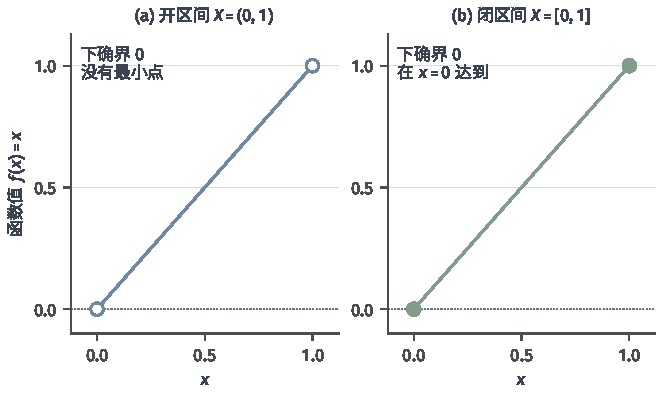
\includegraphics[width=112.0mm]{figures/01-mathematical-preliminaries-upper/01-mathematical-language-combinatorics-analysis-optimization/matplotlib/prelim-minimum-infimum/figure.pdf}
 \caption{同一求值表达式$f(x)=x$在两个定义域上的边界对照。左图定义域为$(0,1)$，空心端点不属于图像，函数值可任意接近$0$，却不能取到；右图定义域为$[0,1]$，实心端点$(0,0)$达到下确界。两图的下确界相同，最小点是否存在取决于可行端点是否保留。图为解析教学示例。}
 \label{fig:prelim-minimum-infimum}
\end{figure}

最小值唯一，最小点却可以有多个。
\begin{example}[同一个最优值可以对应多个输入]
\label{ex:prelim-optimal-value-versus-points}
令$X=[-2,2]$，$f(x)=(x^2-1)^2$。平方非负，且$x=\pm1$都使它为零，所以
\[
 \min_{x\in X}f(x)=\inf_{x\in X}f(x)=0,\qquad \argmin_{x\in X}f(x)=\{-1,1\}.
\]
又因为$0\leq x^2\leq4$，有$|x^2-1|\leq3$，于是$f(x)\leq9$，等号恰在$x=\pm2$处成立，最大值为$9$，最大点集合为$\{-2,2\}$。
\end{example}
例子说明，两个最小点给出的是同一个最小值；最优值相同，并不意味着最优点唯一。怎样求出最小点，是最优化部分的问题，这里只确定它们是什么。
